% $Id: INF_Poster.tex 7714 2011-08-31 17:34:46Z tkren $
%
% TU Wien - Faculty of Informatics
% poster template
%
% This template is using the beamer document class and beamerposter package, see
% <http://www.ctan.org/tex-archive/macros/latex/contrib/beamer/>
% <http://www.ctan.org/tex-archive/macros/latex/contrib/beamerposter/>
% <http://www-i6.informatik.rwth-aachen.de/~dreuw/latexbeamerposter.php>
%
% For questions and comments send an email to
% Thomas Krennwallner <tkren@kr.tuwien.ac.at>
%

\documentclass[final,hyperref={pdfpagelabels=true}]{beamer}

\usepackage{TUINFPST}
\usepackage{lipsum}
\usepackage[position=bottom]{subfig}
\usepackage{caption}

\title[Visual Computing]{Ocean Surface Generation and Rendering}
% if you have a long title looking squeezed on the poster, just force
% some distance:
% \title[Computational Intelligence]{%
%   Integration of Conjunctive Queries over \\[0.2\baselineskip]%
%   Description Logics into HEX-Programs %\\[0.2\baselineskip]%
% }
\author[icicle@cg.tuwien.ac.at]{Thomas Gamper}
\institute[]{%
  Technische Universit{\"a}t Wien\\[0.25\baselineskip]
  Institut f{\"u}r Computergraphik und Algorithmen\\[0.25\baselineskip]
  Arbeitsbereich: Computergraphik\\[0.25\baselineskip]
  BetreuerIn: Assoc. Prof. Dipl.-Ing. Dipl.-Ing. Dr.techn. Michael Wimmer
}
\titlegraphic{
\includegraphics[height=52mm]{186-2}}
\date[\today]{\today}
\subject{epilog}
\keywords{my kwd1, my kwd2}

%%%%%%%%%%%%%%%%%%%%%%%%%%%%%%%%%%%%%%%%%%%%%%%%%%%%%%%%%%%%%%%%%%%%%%%%%%%%%%%%%%%%%%
% Display a grid to help align images 
%\beamertemplategridbackground[1cm]

% for crop marks, uncomment the following line
%\usepackage[cross,width=88truecm,height=123truecm,center]{crop}

%%%%%%%%%%%%%%%%%%%%%%%%%%%%%%%%%%%%%%%%%%%%%%%%%%%%%%%%%%%%%%%%%%%%%%%%%%%%%%%%%%%%%%

\setbeamercolor{block body}{fg=black,bg=white}
\setbeamercolor{block title}{fg=TuWienBlue,bg=white}

\setbeamertemplate{block begin}{
  \begin{flushright}
  \begin{beamercolorbox}{block title}%
    
\begin{tikzpicture}%
      \node[draw,rectangle,line width=3pt,rounded corners,inner sep=0pt]{%
        \begin{minipage}[c][2cm]{\linewidth}
          \centering\textbf{\insertblocktitle}
        \end{minipage}
      };
    \end{tikzpicture}%
  \end{beamercolorbox}
  \vspace*{1cm}
  \begin{beamercolorbox}{block body}%
}

\setbeamertemplate{block end}{
  \end{beamercolorbox}
  \end{flushright}
  \vspace{2cm}
}

%\newenvironment<>{varblock}[2][\textwidth]{
%\begin{center}
% \begin{minipage}{#1}
%  \setlength{\textwidth}{#1}
%  \begin{actionenv}#3
%   \def\insertblocktitle{\centering#2}
%   \par
%   \usebeamertemplate{block begin}}
%   {\par
%       \usebeamertemplate{block end}
%     \end{actionenv}
% \end{minipage}
%\end{center}}

%%%%%%%%%%%%%%%%%%%%%%%%%%%%%%%%%%%%%%%%%%%%%%%%%%%%%%%%%%%%%%%%%%%%%%%%%%%%%%%%%%%%%%
%\setlength{\abovecaptionskip}{-1cm}
%\setlength{\floatsep}{-1cm}
%\setlength{\dblfloatsep}{-1cm}
%\setlength{\intextsep}{-1cm}
%\setlength{\abovecaptionskip}{-1cm}
%\setlength{\belowcaptionskip}{-1cm}
%\captionsetup{skip=-100pt}
\begin{document}

% We have a single poster frame.
\begin{frame}
    \begin{center}
	\begin{minipage}{\textwidth}
		\begin{block}{Introduction}
			\begin{columns}[t]
				\begin{column}{0.45\linewidth}
					\textbf{Motivation}: For computer graphics to reproduce the diverse appearance of ocean
					surfaces represents a sophisticated problem, even more so in the context
					of real-time rendering. The underlying reasons are manifold. First,
					consider the sheer size of  a water body as large as an ocean, which may
					be visible all the way to the horizon. Second, the ocean surface is
					dynamic, therefore it needs to be updated constantly, even though the
					wave interactions that define its shape are huge in terms of complexity.
					Third, the optics of water are intricate. Incoming light may be
					reflected at the surface or may be refracted into the water body. Some
					of the refracted light may even find its way back to the ocean‘s
					surface. Moreover, waves on the surface may break and cause surf and foam.
					
				\end{column}
				\begin{column}{0.45\linewidth}
					\textbf{Problem Statement}:
					The scope of this thesis includes the generation, animation and rendering of the
					surface of an open ocean in real time. We focus our interest on the synthesis of
					animated ocean surface geometry, for which we will adopt a set of models from
					oceanographic research. Specific properties of said models allow for
					easy addition and reduction of detail, as well as for a range of algorithmic
					optimizations. The former combined with the latter gives us the opportunity to
					strike a well-adjusted balance between model detail and computational workload,
					and thereby to improve upon the status quo of current implementations.
				\end{column}	  
%				\begin{column}{0.3\linewidth}
%					\lipsum[3]
%				\end{column}	  
			\end{columns}
		\end{block}
	\end{minipage}
	\begin{minipage}{\textwidth}
		\begin{block}{Ocean Surface Generation}	
			\begin{columns}[t]
				\begin{column}{0.45\linewidth}
					\textbf{Wave Spectra}:
					Phillips, Pierson-Moskowitz, JONSWAP, Donelan, Elfouhaly
				\end{column}
				\begin{column}{0.45\linewidth}
					\textbf{Synthesis}:
					Horizontal and vertical displacements, slopes, first order partial derivatives of the horizontal displacements.
				\end{column}	  
			\end{columns}
		\end{block}
	\end{minipage}
	\begin{minipage}{\textwidth}
		\begin{block}{Ocean Surface Rendering}
			\begin{columns}[t]
				\begin{column}{\linewidth}
				    \begin{figure}
					\centering
%					\noindent
					\subfloat[\label{fig:a}]{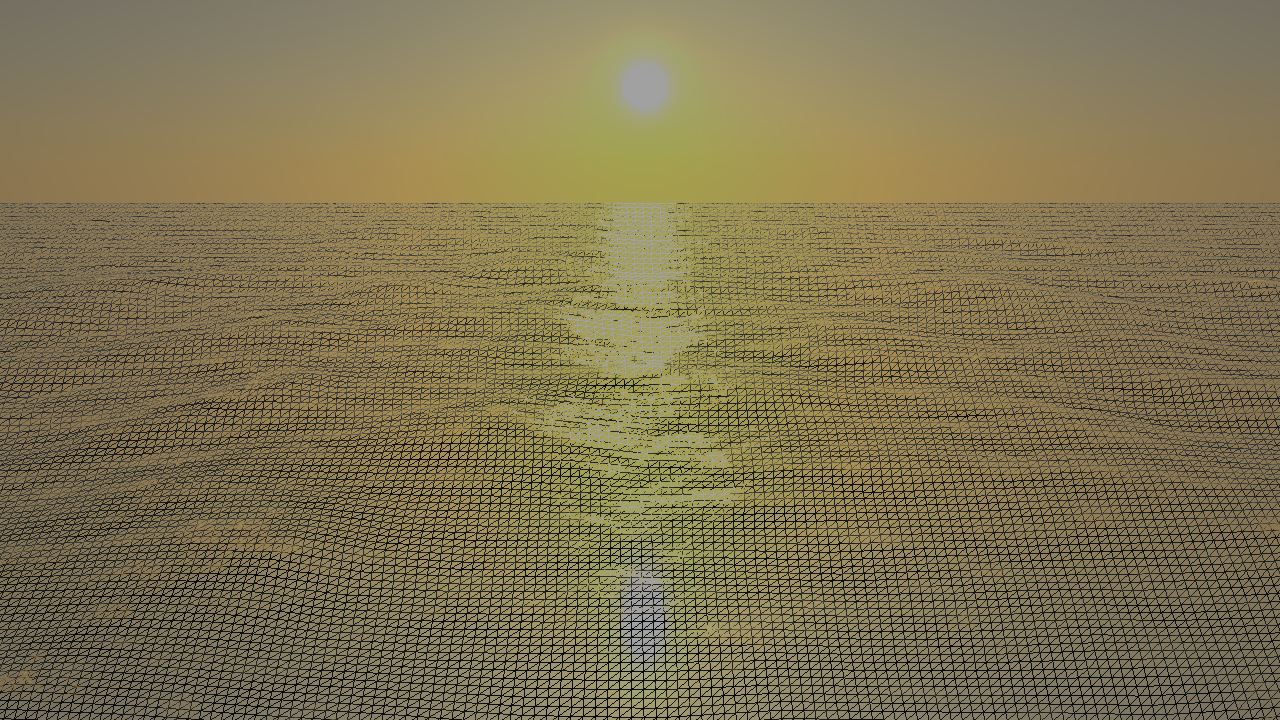
\includegraphics[width=0.165\columnwidth]{figures/28-05-2018_10-56-10_grid}}
					\subfloat[\label{fig:b}]{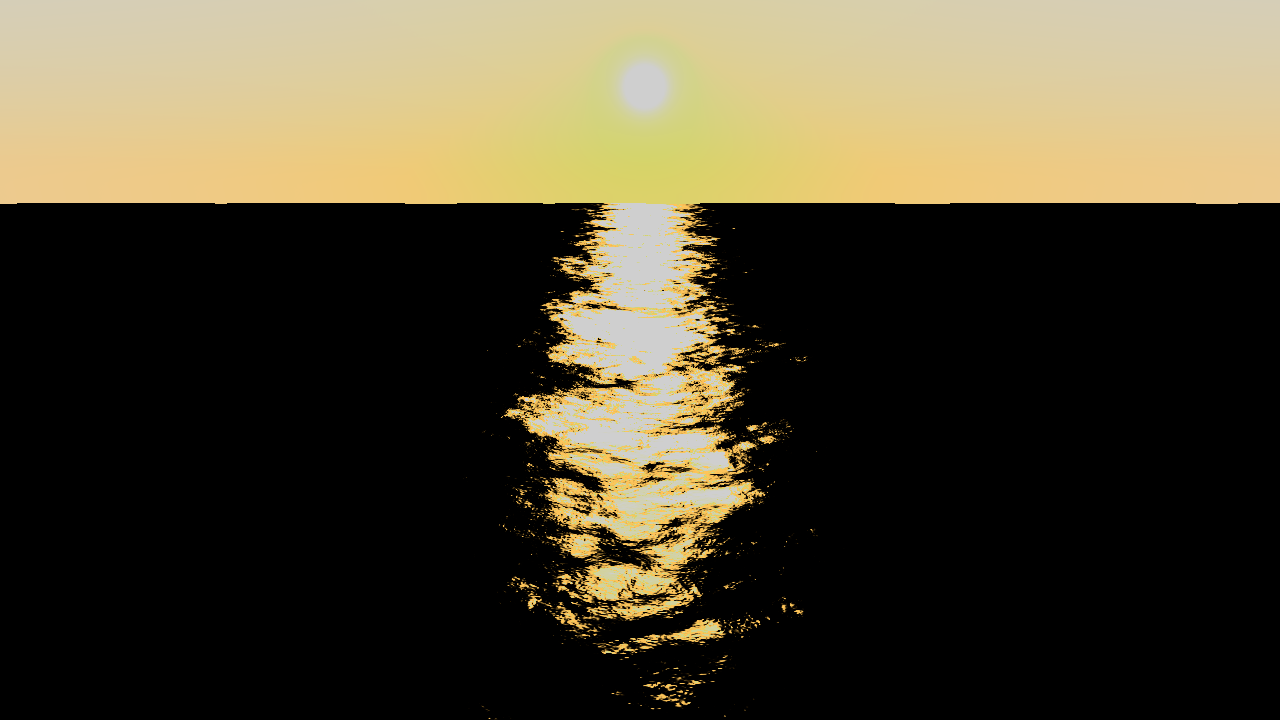
\includegraphics[width=0.165\columnwidth]{figures/28-05-2018_10-56-10_ross}}
					\subfloat[\label{fig:c}]{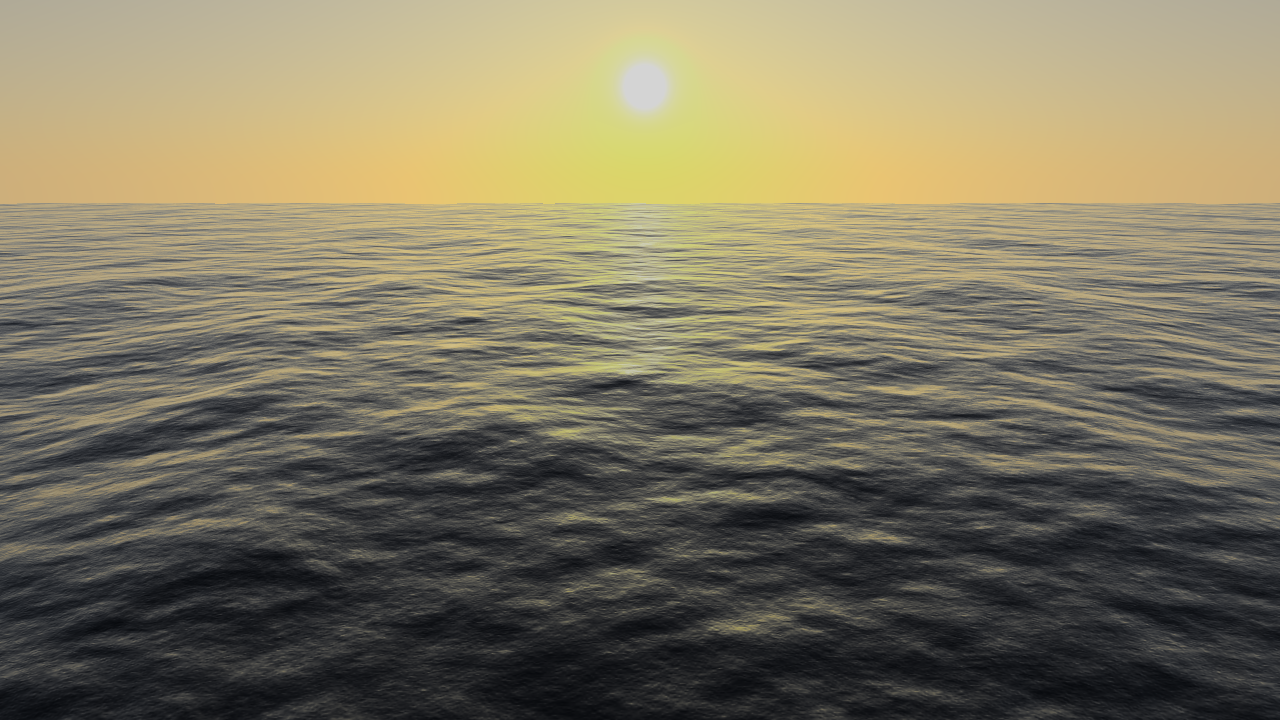
\includegraphics[width=0.165\columnwidth]{figures/28-05-2018_10-56-10_sky}}
					\subfloat[\label{fig:d}]{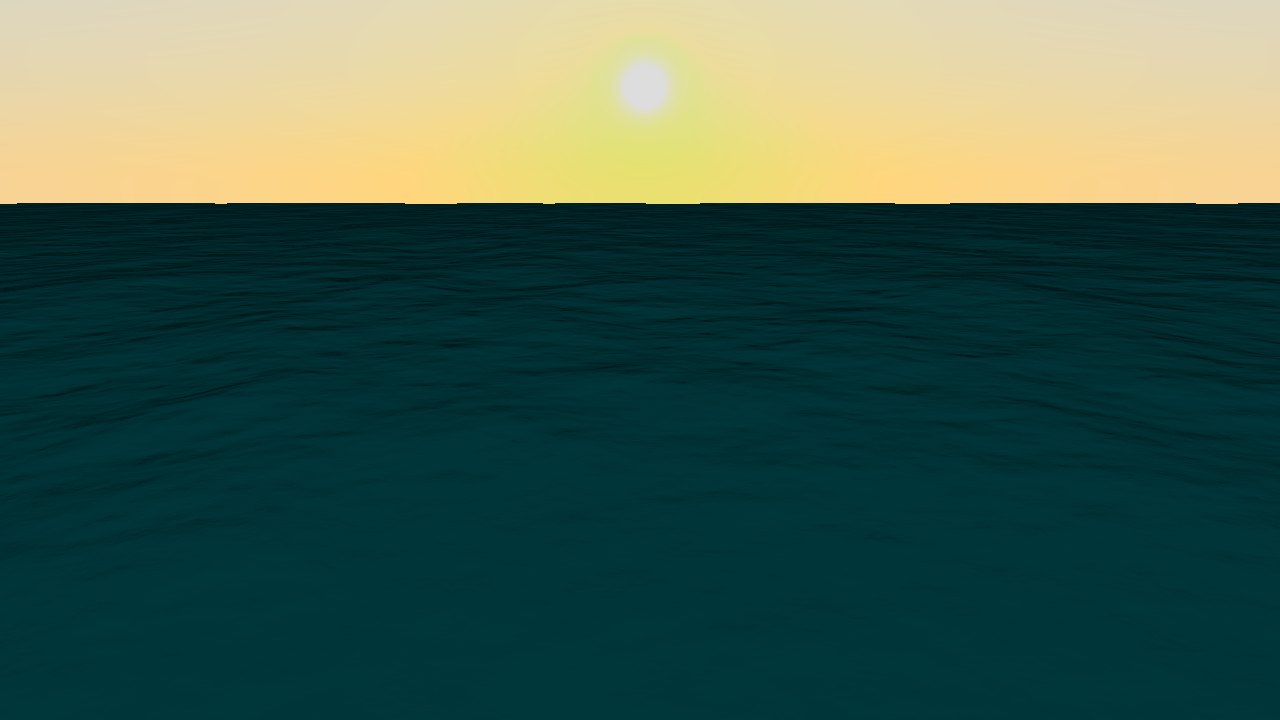
\includegraphics[width=0.165\columnwidth]{figures/28-05-2018_10-56-10_sea}}
					\subfloat[\label{fig:e}]{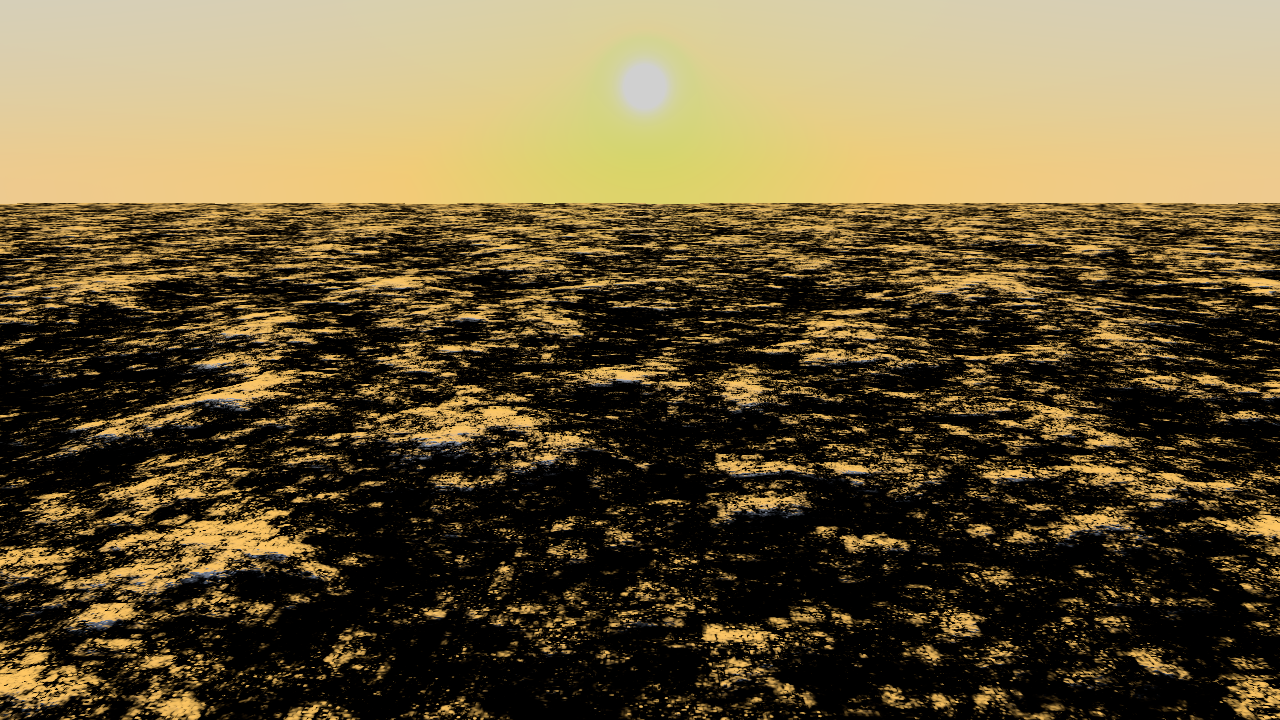
\includegraphics[width=0.165\columnwidth]{figures/28-05-2018_10-56-10_whitecaps}}
					\subfloat[\label{fig:f}]{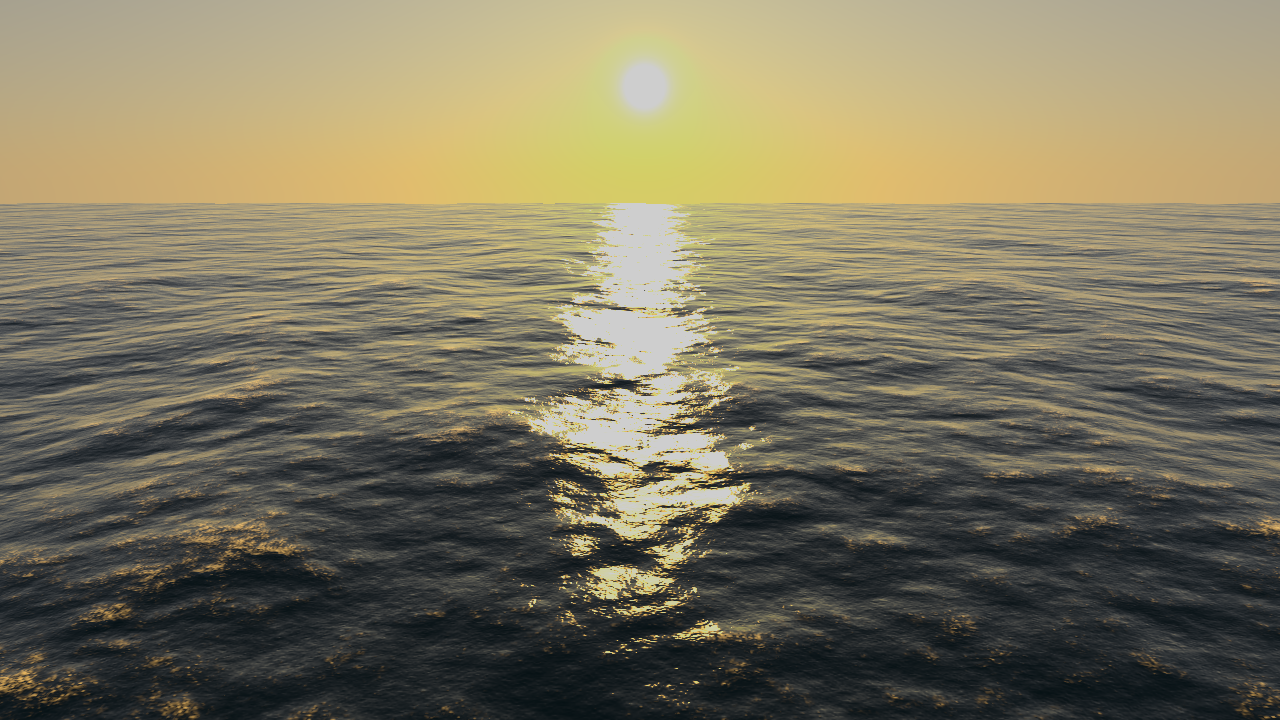
\includegraphics[width=0.165\columnwidth]{figures/28-05-2018_10-56-10_complete}}
					\end{figure}
					\vspace{0.5cm}
					\begin{center}
					From left to right: \subref{fig:a}
					\end{center}
				\end{column}
%				\begin{column}{0.35\linewidth}
%					\subref{fig:a} The adaptive, constant-overhead mesh
%					
%					\subref{fig:b} Sun light reflected by the water surface
%					
%					\subref{fig:c} Sky light reflected by the water surface
%					
%					\subref{fig:d} Light refracted from the water body				
%					
%					\subref{fig:e} Whitecap foam
%					
%					\subref{fig:f} The final result
%				\end{column}				
			\end{columns}
		\end{block}
	\end{minipage}
	\begin{minipage}{\textwidth}
		\begin{block}{Results}
			\begin{columns}[t]
				\begin{column}{0.25\linewidth}
				TROLOLO
				\end{column}
				\begin{column}{0.75\linewidth}
				\begin{center}
%				Brak\cite{ff2010}
				\noindent
				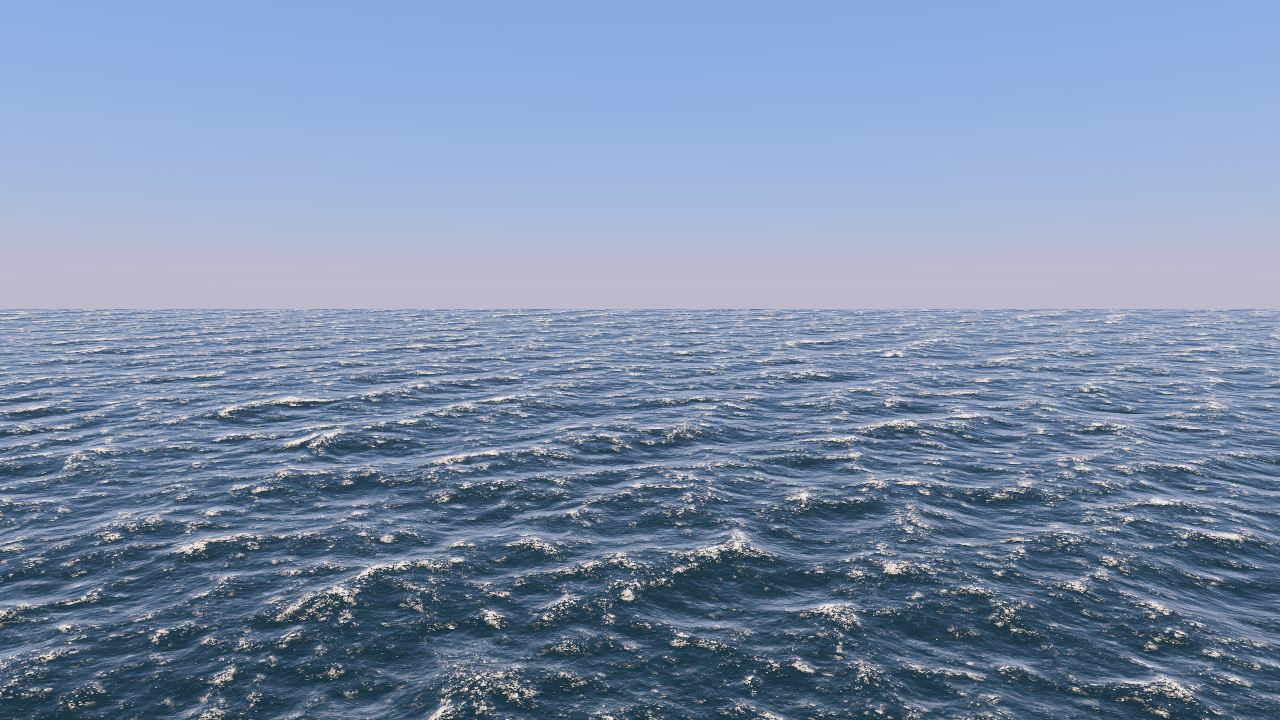
\includegraphics[width=0.225\columnwidth]{figures/21-06-2018_10-44-51_complete}
				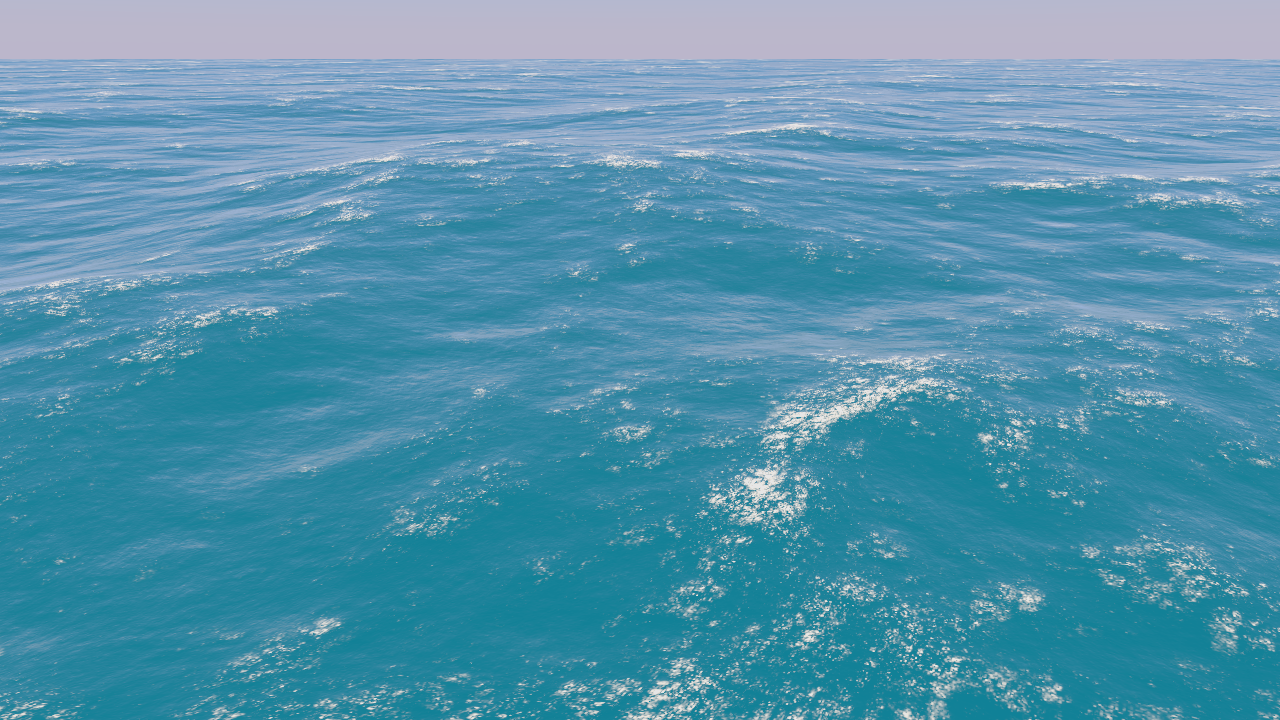
\includegraphics[width=0.225\columnwidth]{figures/21-06-2018_13-45-06_complete}
				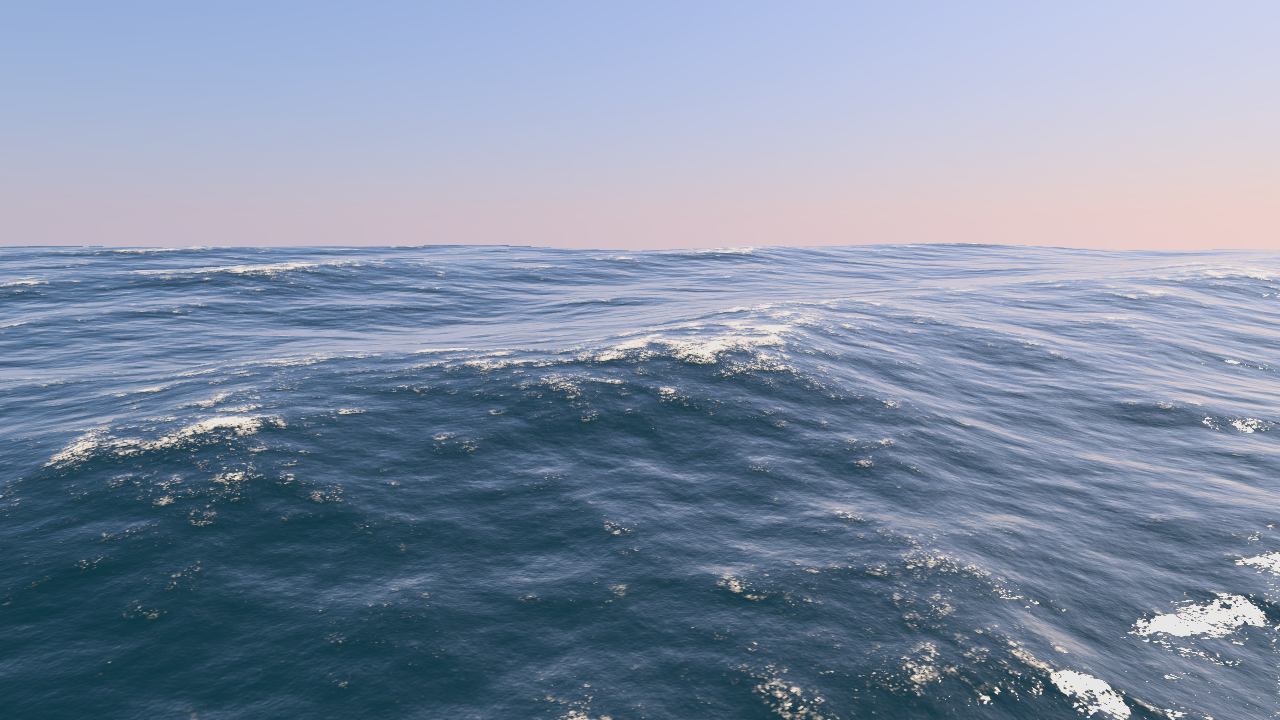
\includegraphics[width=0.225\columnwidth]{figures/21-06-2018_12-48-51_complete}	
				\end{center}
				\end{column}
			\end{columns}
		\end{block}
	\end{minipage}
	\end{center}
%    \begin{varblock}[0.975\textwidth]{Introduction}
%    \end{varblock}
%    \begin{varblock}[0.975\textwidth]{Ocean Surface Generation}
%    Brak
%    \end{varblock}
%    \begin{varblock}[0.975\textwidth]{Ocean Surface Rendering}
%    Brak
%    \end{varblock}
%    \begin{varblock}[0.975\textwidth]{Results}
%    Brak
%    \end{varblock}    
    
%  \begin{columns}[t]
%    % ---------------------------------------------------------%
%    % Set up a column
%    \begin{column}{.45\textwidth}
%      
%    \end{column}
%    % ---------------------------------------------------------%
%    % end the column
%
%    % ---------------------------------------------------------%
%    % Set up a column 
%    \begin{column}{.45\textwidth}
%      
%    \end{column}
%    % ---------------------------------------------------------%
%    % end the column
%  \end{columns}
%
%
%    \begin{thebibliography}{999}
%      
%    \bibitem[Foo~and~Fu, 2010]{ff2010}
%      Foo, B.; and Fu, B.
%      2010.
%      \newblock {On logical representations of hackerisms}.
%      {\em J.~Log.~Hack.} 1:1--2.
%      
%    \bibitem[Crock~et~al., 2010]{ck2010}
%      Crock, A; Cruft, B.; and Kludge, C.
%      2010.
%      \newblock {Decomposing junk code}.
%      Manuscript.
%      
%    \end{thebibliography}

\end{frame}

\end{document}

%%% Local Variables:
%%% TeX-PDF-mode: t
%%% TeX-debug-bad-boxes: t
%%% TeX-master: t
%%% TeX-parse-self: t
%%% TeX-auto-save: t
%%% reftex-plug-into-AUCTeX: t
%%% End:
